\documentclass{beamer}
\usepackage{tikz}
\usetikzlibrary{positioning}

\usefonttheme{professionalfonts}
\usetheme{Boadilla}
\setbeamertemplate{navigation symbols}{}%remove navigation symbols
\hypersetup{pdfstartview={Fit}} % fits the presentation to the window when first displayed

%Info
\title[Detecting Somatic Mutations]{Detection of somatic mutations in \textit{Eucalyptus melliodora}}
\date{3/4/16}
\author{Adam Orr}

% Detection of somatic mutations in *Eucalyptus melliodora*
% =========================================================

% Finding variants (SNPs, insertions, and deletions) is traditionally an involved process
% in which Next-Gen Sequencing reads are compared to a reference, and reads which
% contain changes are reported as variants. In non-model species for which there
% is no genome, this requires *de novo* assembly of a genome. This is computationally expensive
% and time-consuming. New reference-free methods promise fast and accurate detection of of variants.
% I will discuss one such method and evaluate its performance against a traditional pipeline,
% using an individual of the species *Eucalyptus melliodora*. This individual will allow
% us to evaluate phylogenetic tools and has the potential to reveal agriculturally-relevant
% variation. A similar method could be used for understanding the spread of somatic mutations in mammals.

\begin{document}
\frame{\titlepage}
\begin{frame}{About Me}
	\begin{columns}
		\column{.5\linewidth}
			\begin{itemize}
			\item Graduated from ASU with dual major in Math and Molecular Bio
			\item Computational biology in Cartwright lab
			\item Interest in mutation, disease, and evolution
			\item Honors thesis: Database of approximate gene ``ages" using homology and species divergence
			\end{itemize}
		\column{.5\linewidth}
			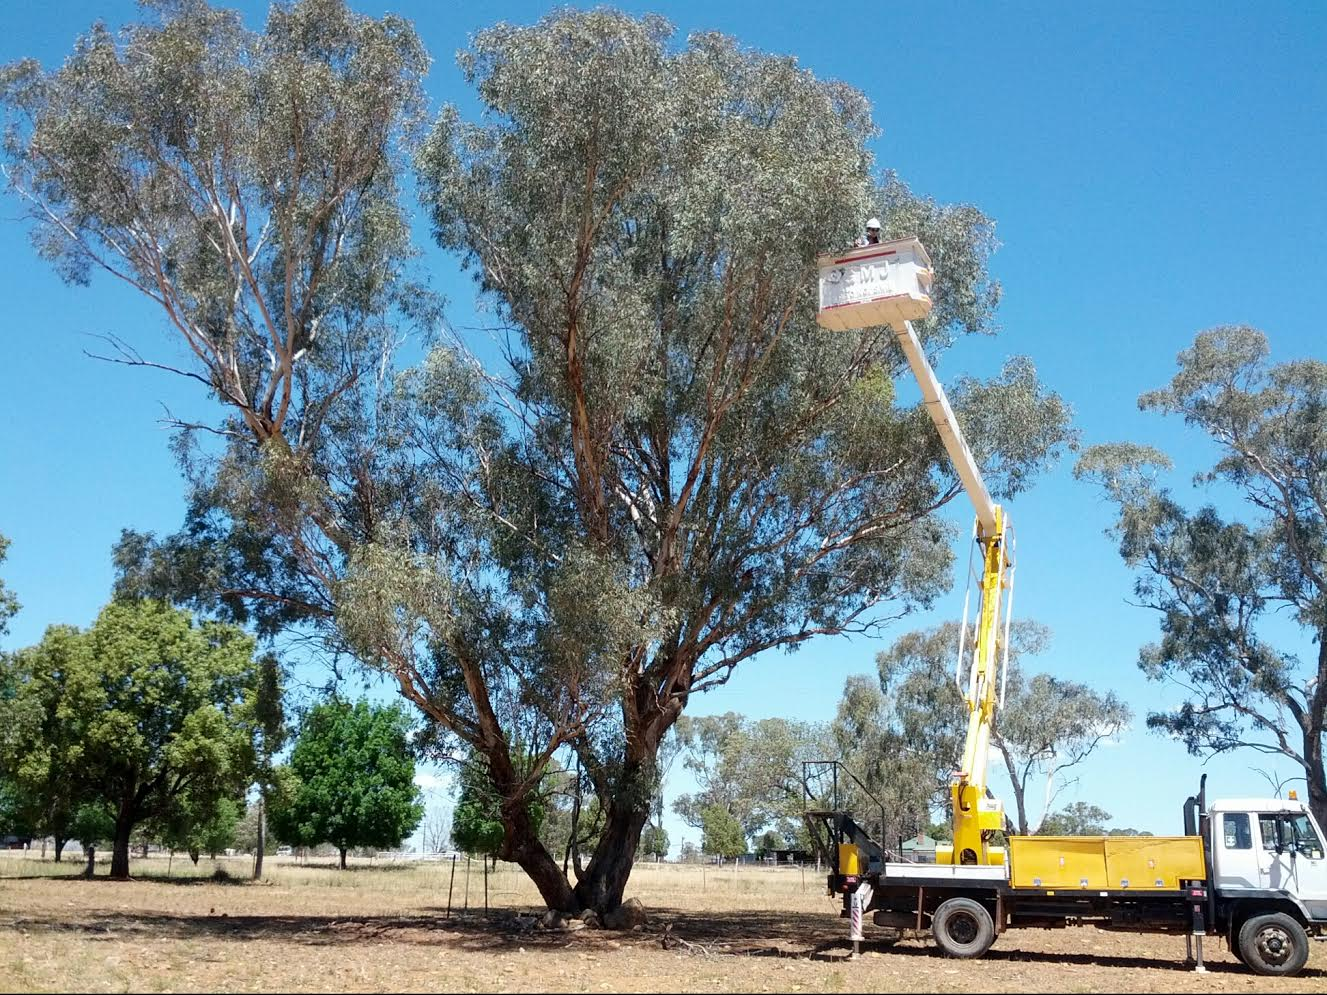
\includegraphics[width=\linewidth]{figures/unlabeled_tree.jpg}
	\end{columns}
\end{frame}

\begin{frame}{Motivation}
	\begin{alertblock}{Remember, a phylogeny is a \textbf{hypothesis}!}
		We use simulations because we can't know the truth \\~\\

		Knowing the truth will allow us to evaluate phylogenetic tools		
	\end{alertblock}

	\begin{definition}
		A \textbf{somatic mutation} is a mutation that occurs in non-germline cells	
	\end{definition}

	\begin{itemize}
	\item How do somatic mutations spread? How can we study this?
	\item Cancers are heterogeneous
	\item Other somatic diseases
	\end{itemize}
\end{frame}

\begin{frame}{A Primer on Next Gen Sequencing}
	\begin{itemize}
	\item Send to the core lab
	\item Get data
	\end{itemize}
\end{frame}

\begin{frame}{Illumina Library Preparation}
	\begin{columns}
		\column{.5\linewidth}
			\begin{itemize}
			\item The advantage of Illumina: massive parallelization
			\item Amplify your DNA
			\item \textbf{Physically} shear your DNA
			\item Add adaptors and inserts to your DNA fragments
			\end{itemize}
		\column{.5\linewidth}
			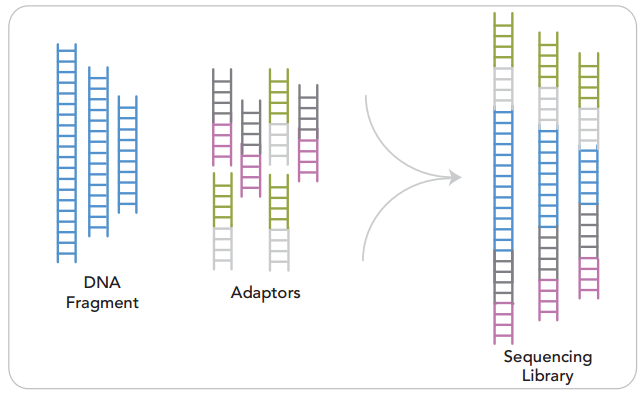
\includegraphics[width=\linewidth]{figures/illumina_library_prep.png}
	\end{columns}
\end{frame}

\begin{frame}{Illumina Sequencing}
	\begin{columns}
		\column{.5\linewidth}
			\begin{itemize}
			\item Adaptor is bound to chip
			\item Bridge amplification
			\item Both strands are bound to chip
			\item Flood with fluorescent nucleotides
			\item Rinse and repeat
			\end{itemize}
			\begin{block}{Follow Me on Instagram}
			Illumina sequencing is a problem of optics. Advances in Illumina sequencing are all fundamentally advances in camera technology. 
			\end{block}
		\column{.5\linewidth}
			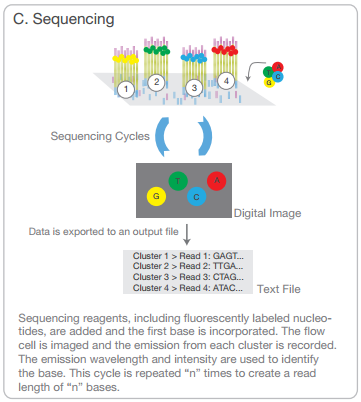
\includegraphics[width=\linewidth]{figures/sequencing.png}
	\end{columns}
\end{frame}

\begin{frame}{Alignment}
	\begin{definition}
	A \textbf{read} is a short (~30bp) segment of sequence determined by the sequencer.
	\end{definition}

	\begin{itemize}
	\item Line up reads to a reference
	\item Some software takes advantage of paired-end technology to improve alignment
	\end{itemize}
	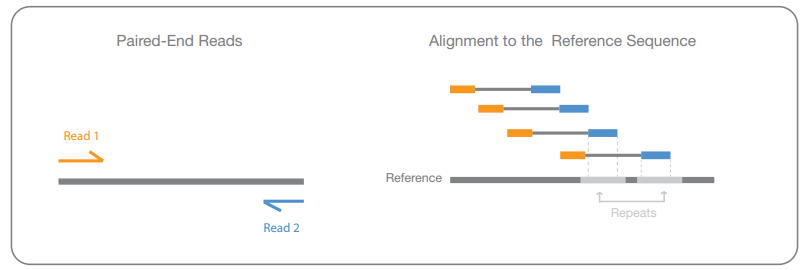
\includegraphics[width=\linewidth]{figures/pe_sequencing.png}
\end{frame}

\begin{frame}{Variant Calling}
	\begin{definition}
	\textbf{Coverage} is the number of reads aligned at a particular position. Large variations in coverage is a symptom of poor alignment or library prep. 
	\end{definition}

	\begin{columns}
		\column{.5\linewidth}
			\begin{itemize}
			\item Account for sequencing error
			\item Variation in sequenced population
			\item Ploidy
			\item Could be Complex algorithm, may be as simple as checking if the base agrees with the reference.
			\end{itemize}
		\column{.5\linewidth}
			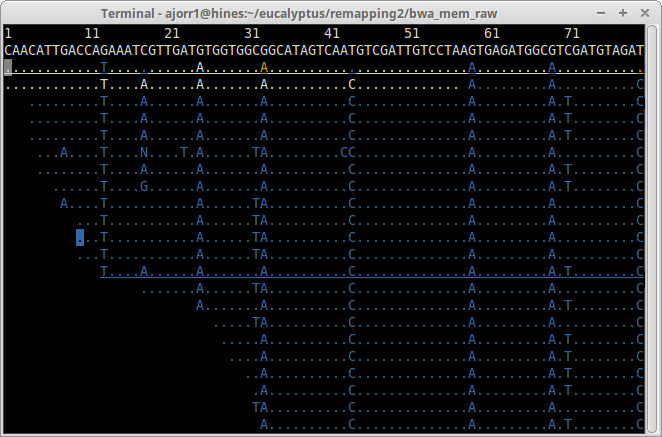
\includegraphics[width=\linewidth]{figures/coverage.png}
	\end{columns}
\end{frame}

\begin{frame}{Assembly}
	\begin{definition}
	A \textbf{contig} is a contiguous stretch of sequence that has been assembled from reads.
	\end{definition}

	\begin{itemize}
	\item Look for overlaps between sequence
	\item Long contig lengths is a sign of a good assembly
	\item Very computationally expensive and time-consuming
	\item Difficult to get right
	\item Contigs are \textbf{not} chromosomes
	\item Sometimes transcript data can be used to join contigs
	\end{itemize}
\end{frame}

\begin{frame}{The Pipeline}
	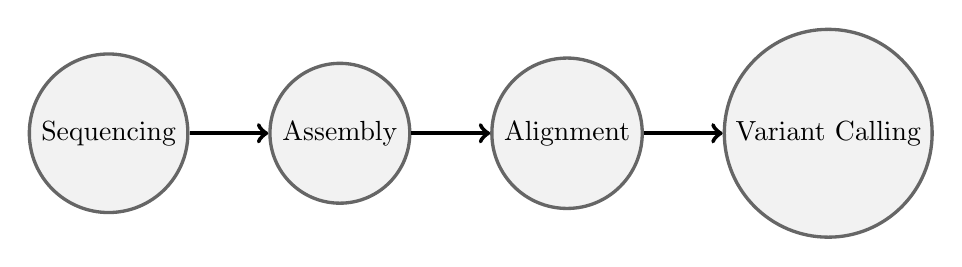
\begin{tikzpicture}[sqnode/.style={circle, draw=black!60, fill=black!5,very thick}]
		\node[sqnode] (sequencing) {Sequencing};
		\node[sqnode] (assembly) [right=of sequencing] {Assembly};
		\node[sqnode] (alignment) [right = of assembly] {Alignment};
		\node[sqnode] (varcall) [right = of alignment] {Variant Calling};
		\draw[ultra thick,->] (sequencing.east) -- (assembly.west);
		\draw[ultra thick,->] (assembly.east) -- (alignment.west);
		\draw[ultra thick,->] (alignment.east) -- (varcall.west);
	\end{tikzpicture}
\end{frame}

\begin{frame}{What if there was a better way?}
	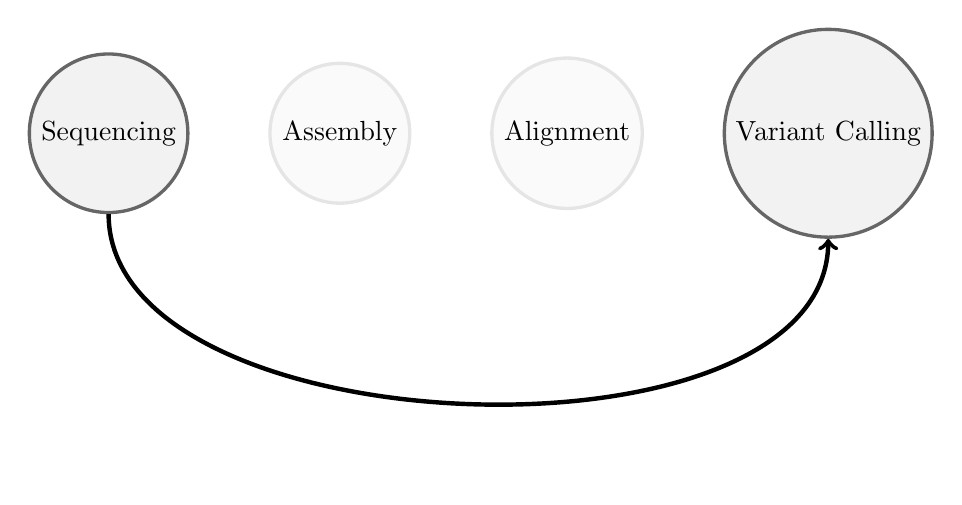
\begin{tikzpicture}[sqnode/.style={circle, draw=black!60, fill=black!5,very thick},lightnode/.style={circle,draw=black!10,fill=black!2,very thick}]
		\node[sqnode] (sequencing) {Sequencing};
		\node[lightnode] (assembly) [right=of sequencing] {Assembly};
		\node[lightnode] (alignment) [right = of assembly] {Alignment};
		\node[sqnode] (varcall) [right = of alignment] {Variant Calling};
		%\draw[ultra thick,->] (sequencing.east) -- (assembly.west);
		%\draw[ultra thick,->] (assembly.east) -- (alignment.west);
		%\draw[ultra thick,->] (alignment.east) -- (varcall.west);
		\draw[ultra thick,->] (sequencing.south) .. controls +(down:30mm) and +(down:30mm) .. (varcall.south);
	\end{tikzpicture}
\end{frame}

\begin{frame}{What is a graph?}
	\begin{definition}
	A \textbf{graph} is a set of nodes and a set of edges, G = (V,E)
	\end{definition}
	\centering
	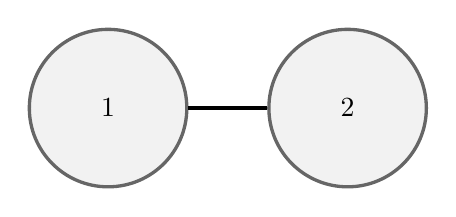
\begin{tikzpicture}[cnode/.style={circle, draw = black!60, fill=black!5,very thick, minimum size = 20mm}]
		\node[cnode] (leftnd) {1};
		\node[cnode] (rightnd) [right = of leftnd]{2};
		\draw[very thick] (leftnd.east) -- (rightnd.west);
	\end{tikzpicture}

	V = \{1 , 2\}

	E = \{(1,2)\}

\end{frame}

\begin{frame}{The De Bruijn Graph}
	\begin{definition}
	A \textbf{De Bruijn Graph} is a graph where the nodes represent symbols and edges represent overlaps between those symbols.
	\end{definition}

	De Bruijn Graphs are \textbf{Eulerian}

	\begin{definition}
	A \textbf{Eulerian} graph is a graph in which each edge is visited once.
	\end{definition}

	\begin{example}
	Consider the sequence \textbf{AATGCAT} and split it with \textbf{kmer} size 3

	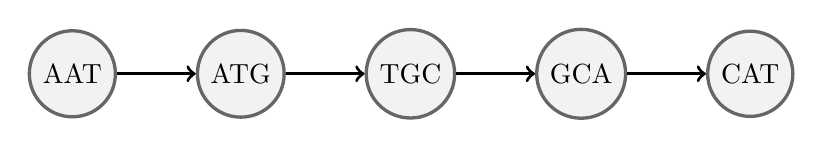
\begin{tikzpicture}[cnode/.style={circle,draw=black!60,fill=black!5,very thick}]
		\node[cnode] (aat) {AAT};
		\node[cnode] (atg) [right = of aat] {ATG};
		\node[cnode] (tgc) [right = of atg] {TGC};
		\node[cnode] (gca) [right = of tgc] {GCA};
		\node[cnode] (cat) [right = of gca] {CAT};
		\draw[very thick,->] (aat.east) -- (atg.west);
		\draw[very thick,->] (atg.east) -- (tgc.west);
		\draw[very thick,->] (tgc.east) -- (gca.west);
		\draw[very thick,->] (gca.east) -- (cat.west);
	\end{tikzpicture}
	\end{example}

\end{frame}

\begin{frame}{Calling Variants Using Bubbles}
What happens when your pooled sample contains a mutant?

\begin{example}
Consider the sequence \textbf{AATGCAT} and split it with \textbf{kmer} size 3.
There is a sample with a G to C mutation!


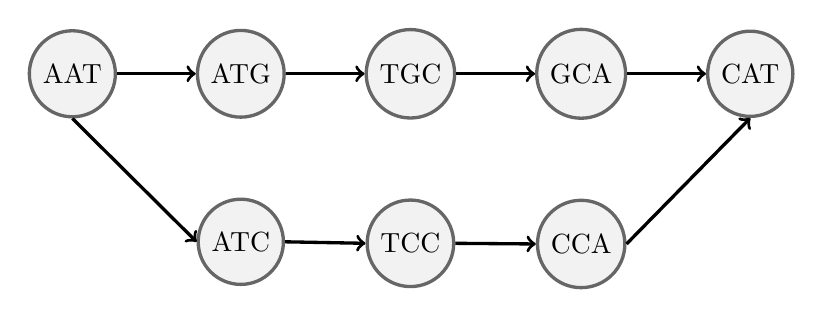
\begin{tikzpicture}[cnode/.style={circle,draw=black!60,fill=black!5,very thick}]
	\node[cnode] (aat) {AAT};
	\node[cnode] (atg) [right = of aat] {ATG};
	\node[cnode] (tgc) [right = of atg] {TGC};
	\node[cnode] (gca) [right = of tgc] {GCA};
	\node[cnode] (cat) [right = of gca] {CAT};
	\node[cnode] (atc) [below = of atg] {ATC};
	\node[cnode] (tcc) [below = of tgc] {TCC};
	\node[cnode] (cca) [below = of gca] {CCA};
	\draw[very thick,->] (aat.east) -- (atg.west);
	\draw[very thick,->] (atg.east) -- (tgc.west);
	\draw[very thick,->] (tgc.east) -- (gca.west);
	\draw[very thick,->] (gca.east) -- (cat.west);
	\draw[very thick,->] (aat.south) -- (atc.west);
	\draw[very thick,->] (atc.east) -- (tcc.west);
	\draw[very thick,->] (tcc.east) -- (cca.west);
	\draw[very thick,->] (cca.east) -- (cat.south);
\end{tikzpicture}
\end{example}

This is a \textbf{bubble}. Bubbles of the same size as the kmer size are indicative of a mutation.

\end{frame}

\begin{frame}{Back to \textit{Eucalyptus}}
	\begin{itemize}
	\item Reference-free De Bruijn variant caller \textbf{DiscoSNP++}
	\item 8 samples, each with 3 replicates
	\item Protect against false positive by forcing replicates to agree
	\end{itemize}
	\begin{columns}
	\column{.5\linewidth}
		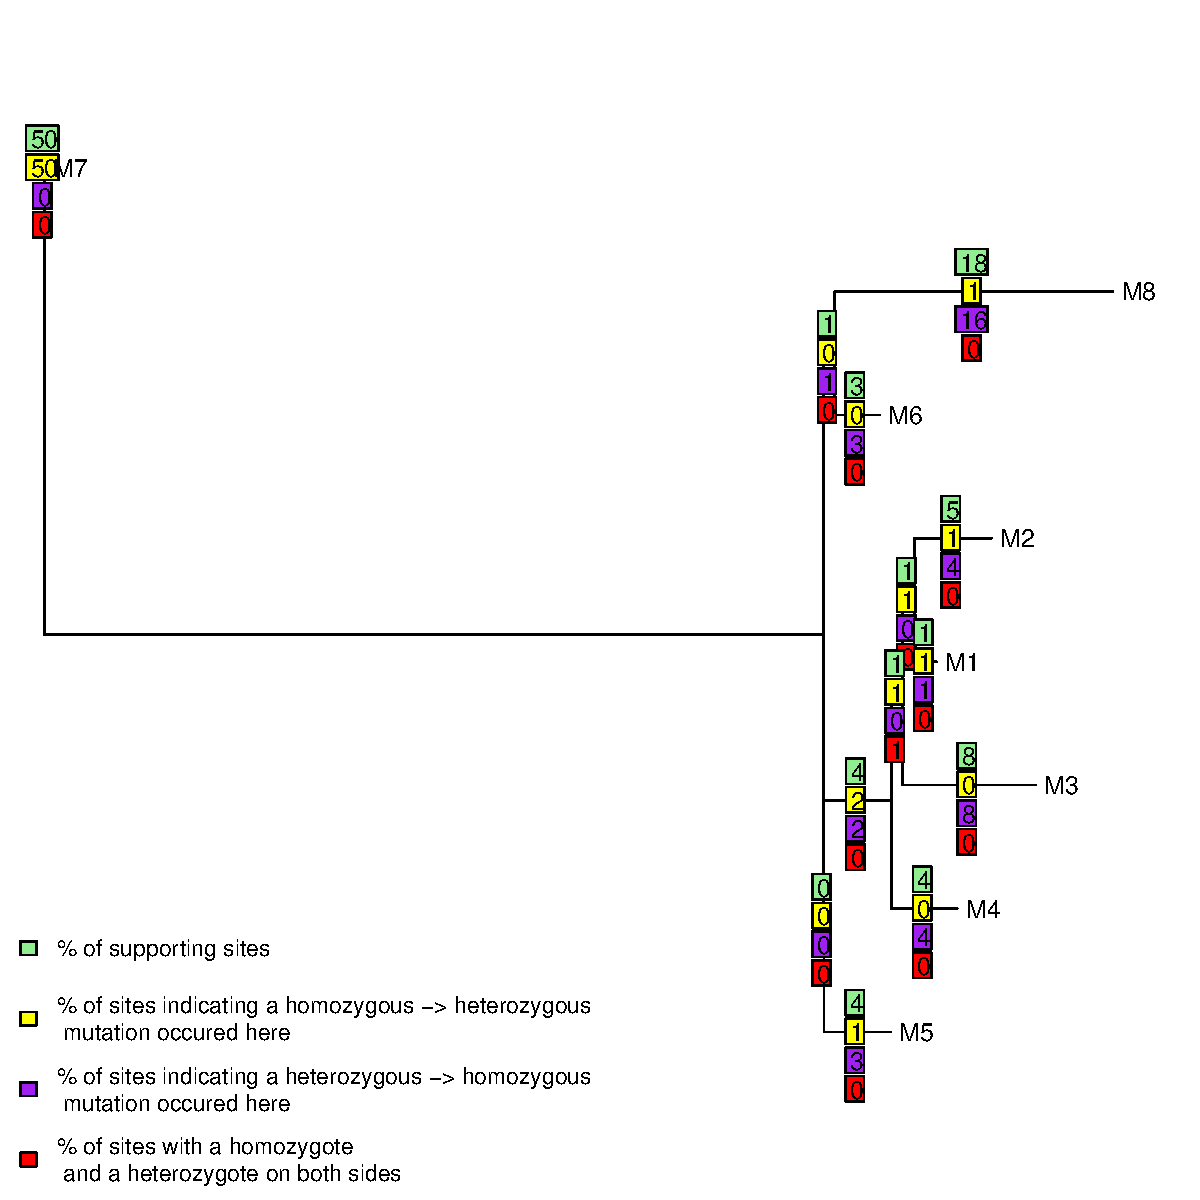
\includegraphics[width=\linewidth]{figures/disco_tree.pdf}
	\column{.5\linewidth}
		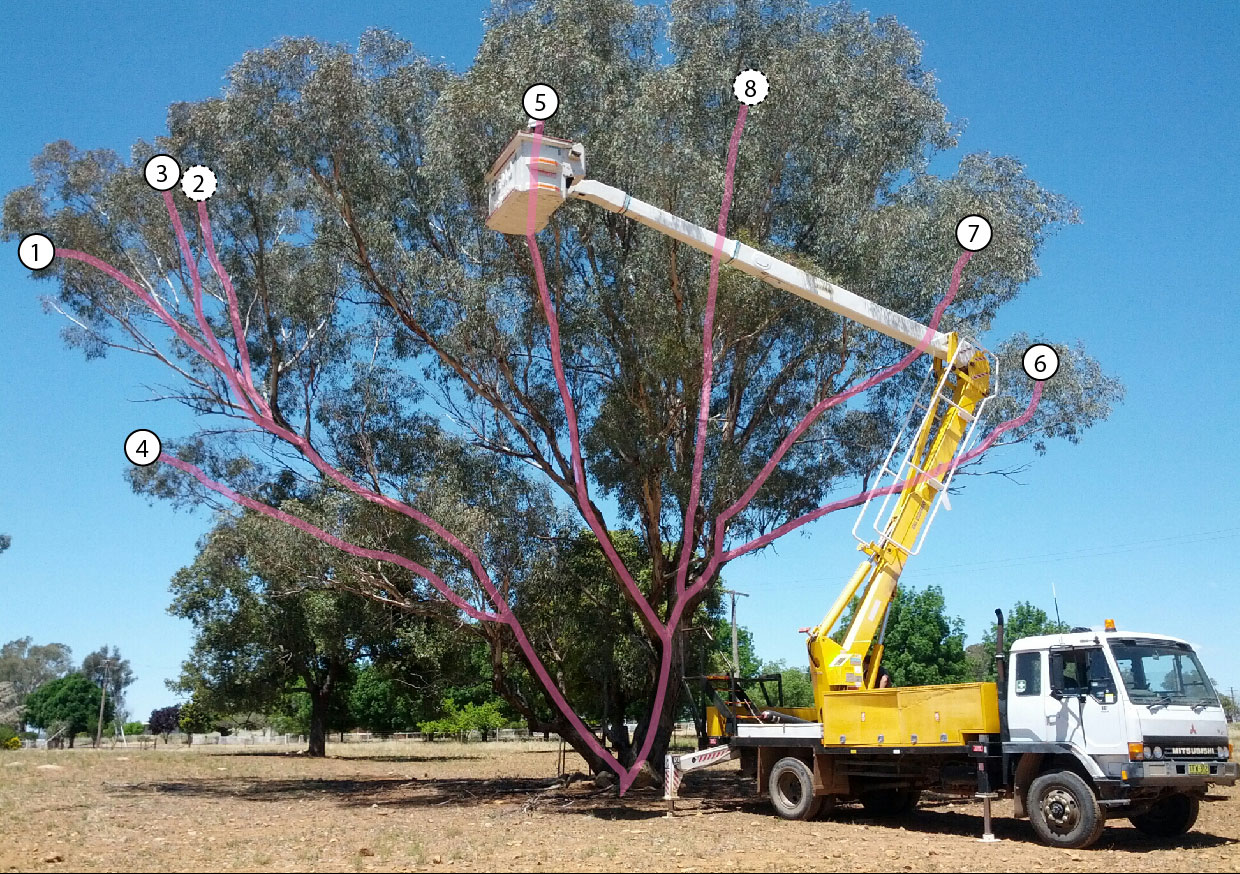
\includegraphics[width=\linewidth]{figures/labeled_tree.jpg}
	\end{columns}
\end{frame}

\begin{frame}{The Genome Analysis Toolkit}
	\begin{itemize}
	\item Used a traditional variant-calling pipeline: GATK best practices workflow
	\item Reference genome of a close relative: \textit{Eucalyptus Grandis}
	\end{itemize}
	\begin{columns}
	\column{.5\linewidth}
		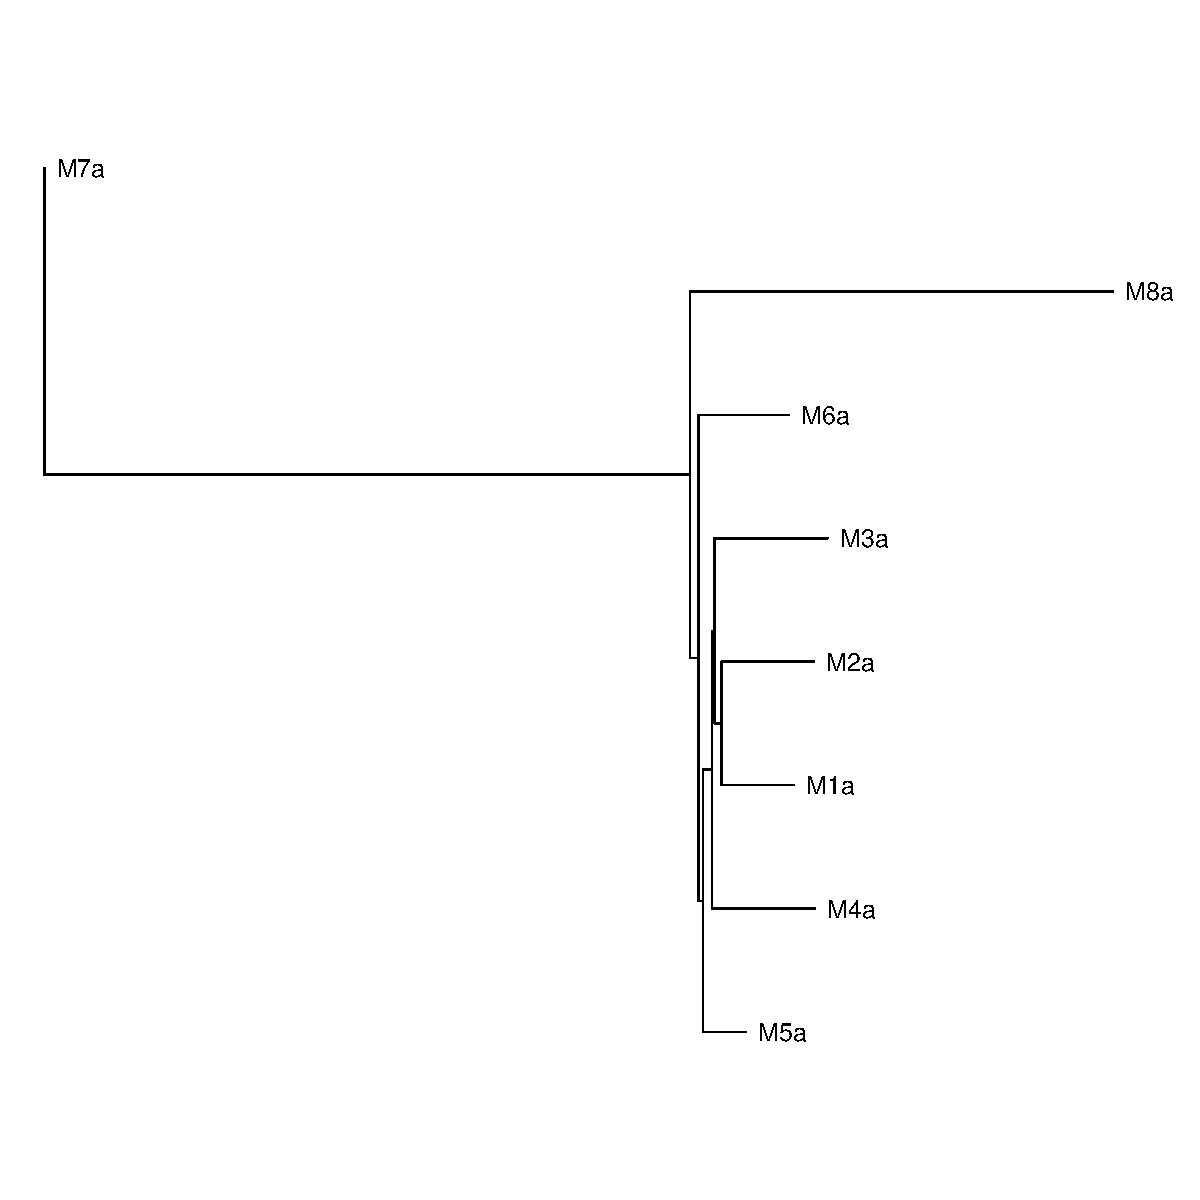
\includegraphics[width=\linewidth]{figures/gatk_tree.pdf}
	\column{.5\linewidth}
		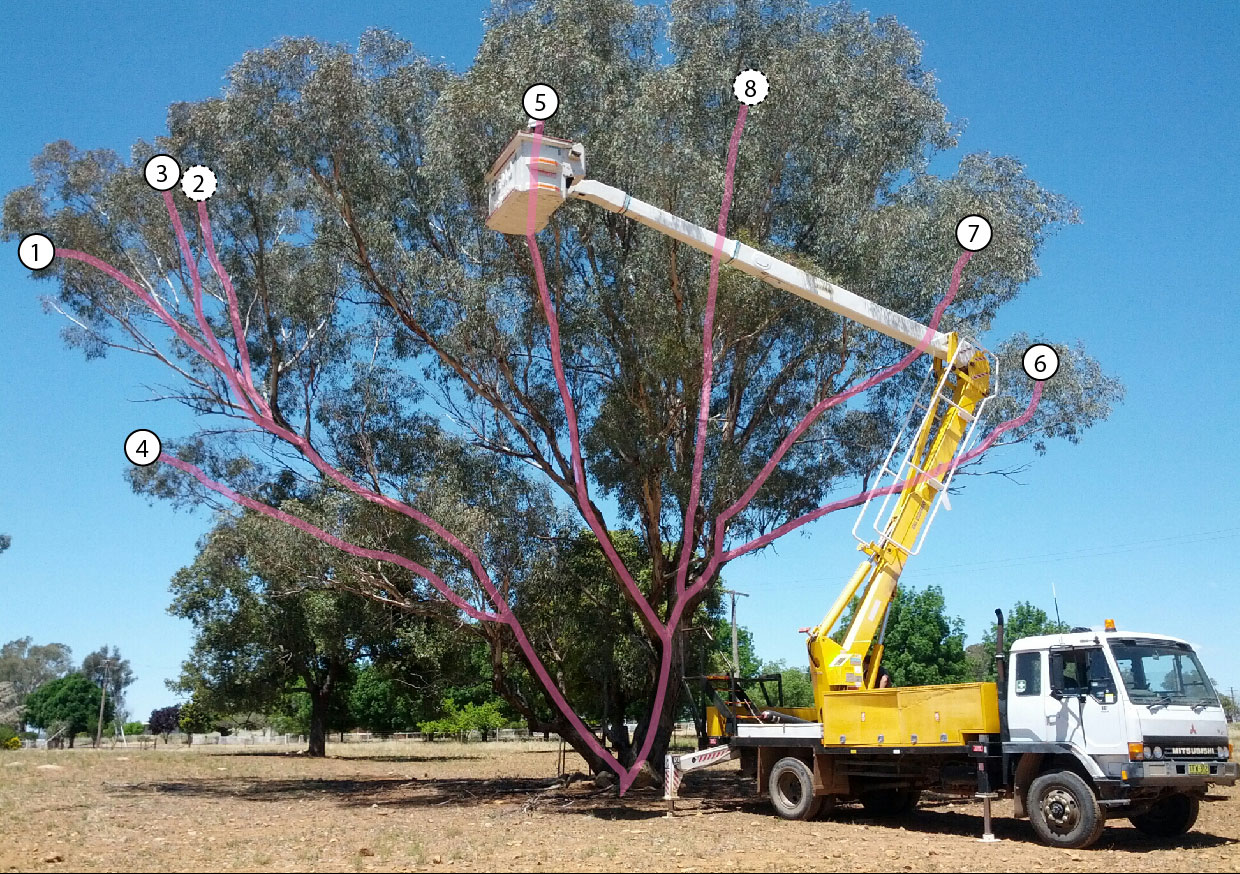
\includegraphics[width=\linewidth]{figures/labeled_tree.jpg}
	\end{columns}
\end{frame}

\begin{frame}{What's going on here?}
Branch 7 is consistently in the wrong place. Why? What's going on with that branch?
\begin{itemize}
\item Branch 7 is the longest branch
\item May do with assumptions about zygosity
\item Recursively improving alignment with various tools
\end{itemize}
\end{frame}

\begin{frame}{Acknowledgements}
\begin{itemize}
\item Advisor Reed Cartwright
\item Collaborator Robert Lanfear
\end{itemize}
\end{frame}

%Graph Theory
%How does a reference free method work?
%The tree I got
%Compare to GATK
%Why is this happening? IDK
%Talk about improving the assembly

\end{document}